\documentclass[11pt, twoside]{article}

% [final] muestra autores y quita la numeración de líneas de revisión de ACL
\usepackage[final]{acl}
\setlength{\titlebox}{9\baselineskip}
\usepackage{times}
\usepackage{latexsym}
\usepackage[T1]{fontenc}
\usepackage[utf8]{inputenc}
\usepackage[spanish,es-tabla]{babel}
\usepackage{microtype}
\usepackage{inconsolata}
\usepackage{graphicx}
\usepackage{booktabs}
\usepackage{amsmath}
\usepackage{url}
\usepackage{etoolbox}
\usepackage{enumitem}
\usepackage{multirow}
\usepackage{tikz}
\usetikzlibrary{positioning,arrows.meta,fit,backgrounds}
\captionsetup[figure]{font=small}
\captionsetup[table]{font=small}

\setlength{\textfloatsep}{16pt plus 2pt minus 2pt}
\setlength{\intextsep}{10pt plus 2pt minus 2pt}
\setlength{\dbltextfloatsep}{16pt plus 2pt minus 2pt}
\makeatletter
\renewcommand{\paragraph}{\@startsection{paragraph}{4}{\z@}{2.0ex plus 0.7ex minus 0.3ex}{-1em}{\normalsize\bfseries}}
\makeatother
\makeatletter
\patchcmd{\thebibliography}{References}{Referencias}{}{}
\patchcmd{\thebibliography}{References}{Referencias}{}{}
\patchcmd{\thebibliography}{References}{Referencias}{}{}
\makeatother

\newcommand{\topic}[1]{\texttt{\small #1}}

\title{Interpretación y Representación Semántica del Entorno}

\author{
  \textbf{Stefania Bianchi Morales, Sara Mora García,}\\
  \textbf{Alejandro Operé Sirvent, Celia Ribes Flor}\\[0.3cm]
  Universidad de Alicante\\
  \texttt{\{sbm108, smg200, aos35, crf41\}@alu.ua.es}
}

\usepackage{fancyhdr}

%===============================================================================
%                            ENCABEZADO Y PIE
%===============================================================================

\pagestyle{fancy}
\fancyhf{}

\fancyhead[LO]{\footnotesize \bfseries ROBÓTICA INTELIGENTE}
\fancyhead[RO]{\footnotesize Diciembre de 2026}

\fancyhead[LE]{\footnotesize Interpretación y Representación Semántica del Entorno / \scriptsize S. BIANCHI, S. MORA, A. OPERÉ, C. RIBES}

\cfoot{\thepage}

\renewcommand{\headrulewidth}{0pt}

\fancypagestyle{firstpage}{
\fancyhf{}
\fancyhead[LO]{\footnotesize \bfseries ROBÓTICA INTELIGENTE}
\fancyhead[R]{\footnotesize Diciembre de 2026}
\cfoot{\thepage}
\renewcommand{\headrulewidth}{0pt}
}

\begin{document}

\maketitle
\thispagestyle{firstpage}

\begin{abstract}
Presentamos un sistema en ROS~2 que construye mapas semánticos 3D de entornos urbanos a partir de un LiDAR, una IMU y tres cámaras ojo de pez del Oxford Spires Dataset. La odometría LiDAR-inercial RKO-LIO proporciona la trayectoria; un modelo de segmentación preentrenado (SegFormer, Cityscapes) etiqueta las imágenes en la GPU; cada punto del LiDAR se proyecta sobre la cámara que lo ve con menos distorsión mediante el modelo equidistante calibrado, y las etiquetas se fusionan en un mapa voxelizado con votación bayesiana. Sobre la secuencia Keble College~01 (289\,m, 5\,min), la odometría obtiene un ATE de 11,2\,cm frente a la trayectoria de referencia del dataset, y el mapa resultante (2,8\,M voxels de 15\,cm) queda etiquetado en su totalidad con una confianza media del 95,5\,\%. La comparación con YOLO11-seg muestra que la detección de objetos solo cubre el 0,6\,\% del mapa, lo que justifica la segmentación densa. Todo el sistema se reproduce con un único comando en el contenedor Docker de la asignatura.
\end{abstract}

%==========================================================
\section{Introducción}
%==========================================================
La robótica móvil de exteriores ha pasado de la navegación puramente geométrica, centrada en evitar colisiones, a la comprensión del contexto en el que opera el robot. Un mapa métrico indica \emph{dónde} hay estructura, pero no \emph{qué} es: un edificio, un árbol o un vehículo aparcado se representan igual en una nube de puntos. Esta carencia limita la planificación de alto nivel, la interacción con clases concretas del entorno y la reutilización del mapa por otros módulos del sistema.

Este proyecto aborda el problema combinando dos tecnologías complementarias. La primera es la odometría LiDAR-inercial (LIO), que aporta una trayectoria precisa y una reconstrucción 3D consistente. La segunda es la visión por computador basada en modelos preentrenados de gran escala, que aporta información semántica densa sin entrenar redes desde cero. Como base geométrica se emplea RKO-LIO, un sistema que no requiere modelado específico del sensor y funciona en distintas plataformas y entornos sin cambiar la configuración~\cite{malladi2026rkolio}. Como fuente de datos se usa el Oxford Spires Dataset (OSD), que cubre seis edificios históricos de Oxford con 24 secuencias e incluye tres cámaras RGB de obturador global, un LiDAR de 64 haces e inercial, junto con modelos 3D de referencia de precisión milimétrica obtenidos con un escáner láser terrestre~\cite{tao2024spires}.

El objetivo principal es construir un mapa 3D etiquetado del entorno urbano. Para ello, se segmentan las imágenes con modelos de visión preentrenados y se proyectan las etiquetas resultantes sobre la nube de puntos generada por la odometría.

El desarrollo de esta arquitectura se fundamenta en tres motivos principales:
\begin{enumerate}[noitemsep]
  \item Aborda un problema abierto de gran relevancia actual, respaldado por la intensa actividad investigadora en mapas semánticos y representaciones 3D para robótica~\cite{firoozi2023foundation,deng2025best3d}.
  \item Se integra de manera robusta sobre estándares de facto en la industria y conjuntos de datos de última generación (ecosistema ROS~2, arquitecturas LIO, OSD).
  \item Permite una evaluación rigurosa tanto cuantitativa como cualitativa, dado que el conjunto de datos proporciona referencias geométricas (\emph{ground truth}) de muy alta precisión.
\end{enumerate}

Las contribuciones de este trabajo son:
\begin{enumerate}[noitemsep]
  \item Un \emph{pipeline} modular en ROS~2 (tres nodos propios más RKO-LIO) que proyecta las etiquetas 2D de tres cámaras ojo de pez sobre el LiDAR y las fusiona en un mapa voxelizado en tiempo real.
  \item Una evaluación cuantitativa sobre la secuencia Keble College~01: precisión de la odometría frente a la referencia del OSD, composición y confianza del mapa semántico, y tiempos de cómputo por nodo.
  \item Una comparación entre segmentación semántica densa (SegFormer) y segmentación de instancias de objetos (YOLO11-seg) para este problema.
  \item Un entorno reproducible con un único comando sobre el contenedor Docker de la asignatura con soporte de GPU.
\end{enumerate}

%==========================================================
\section{Estado del Arte}
%==========================================================

\subsection{Odometría LiDAR-inercial y conjuntos de datos de referencia}

Los sistemas LIO fusionan nubes de puntos e IMU, bien mediante filtros, bien mediante grafos de factores. RKO-LIO incorpora un esquema de regularización adaptativa en el registro ICP y se publica en \emph{IEEE Robotics and Automation Letters}~\cite{malladi2026rkolio}. Sobre este tipo de trayectorias se construyen los mapas semánticos, de modo que su calidad condiciona directamente el etiquetado final.

Para evaluar estos métodos, el OSD se plantea como banco de pruebas de localización, reconstrucción y síntesis de nuevas vistas en exteriores a gran escala. Según sus autores, no existía hasta entonces un conjunto con imágenes en color, LiDAR y trayectoria y reconstrucción de referencia precisas~\cite{tao2024spires}. Esto lo hace adecuado para mapeo semántico, aunque el dataset \emph{no incluye anotaciones semánticas}. La evaluación semántica deberá apoyarse, por tanto, en etiquetado manual parcial o en métricas indirectas.

\subsection{Mapas semánticos 3D: de lo geométrico a lo etiquetado}

Los primeros mapas semánticos 3D dependían de la cámara tanto para reconstruir como para etiquetar. Jeong et~al. señalan que estos enfoques sufrían limitaciones y no trataban los rastros de vehículos en movimiento, y proponen combinar LiDAR y cámara para escalas grandes~\cite{jeong2018towards}. Su sistema integra el mapa 3D con la información semántica mediante transformación de coordenadas y actualización bayesiana, y añade un refinamiento para corregir voxeles mal segmentados y eliminar las huellas de vehículos móviles. Este trabajo adopta dicho esquema: segmentación 2D, proyección, fusión probabilística por voxel y refinamiento.

Para representar el mapa, OctoMap sigue siendo la referencia volumétrica. Se basa en octrees con estimación probabilística de ocupación y representa explícitamente el espacio ocupado, libre y desconocido~\cite{hornung2013octomap}. OctoMap modela ocupación, no semántica, por lo que el etiquetado se añade como extensión mediante la actualización bayesiana por voxel descrita arriba. En paralelo, Kimera integra SLAM visual-inercial, optimización de grafo de poses y una malla 3D anotada semánticamente a partir de segmentación 2D píxel a píxel~\cite{rosinol2020kimera}.

\subsection{Segmentación directa 3D frente a proyección desde imagen}

Existen dos estrategias para etiquetar nubes de puntos. La primera segmenta la nube directamente con redes 3D. Zou et~al. adaptan ARandLA-Net a un conjunto urbano de unos 390 millones de puntos de escaneo láser móvil, con un mIoU del 54,4\,\% y una mejora aproximada del 4\,\% al incorporar color~\cite{zou2021towards}. Esta vía depende de datos anotados en 3D, escasos y costosos.

La segunda estrategia proyecta los puntos sobre imágenes ya segmentadas. Ochs et~al. comparan ambas y observan que proyectar el LiDAR sobre la segmentación de la cámara mejora la localización sin necesidad de segmentar directamente la nube~\cite{ochs2025boosting}. Es la vía más adecuada para este proyecto, pues aprovecha la madurez de la segmentación 2D y no exige anotaciones 3D.

\subsection{Modelos de visión preentrenados y fundacionales}

YOLO plantea la detección como una regresión directa de cajas delimitadoras y probabilidades de clase en una única evaluación de red, a 45 fps en su versión base~\cite{redmon2016yolo}. Sus versiones actuales, como YOLO11~\cite{jocher2024yolo11}, añaden máscaras de instancia y se entrenan sobre las 80 clases de COCO~\cite{lin2014coco}. Es adecuado para objetos discretos (vehículos, señales) y para ejecución en tiempo real, pero COCO no contiene clases de escena como edificio, vegetación o calzada.

La segmentación semántica densa asigna una clase a cada píxel. SegFormer combina un codificador \emph{transformer} jerárquico sin codificación posicional con un decodificador ligero de perceptrones, y obtiene resultados de referencia en Cityscapes con un coste moderado~\cite{xie2021segformer}. Cityscapes define 19 clases de escena urbana (calzada, acera, edificio, vegetación, terreno, señal, vehículos\ldots)~\cite{cordts2016cityscapes}, que coinciden con las que pide este proyecto.

Segment Anything (SAM) introduce una tarea de segmentación \emph{promptable}, un modelo con transferencia \emph{zero-shot} y el conjunto SA-1B, con más de mil millones de máscaras sobre 11 millones de imágenes~\cite{kirillov2023sam}. Sus máscaras son de calidad, pero \emph{no llevan etiqueta de clase}, por lo que suele combinarse con un detector o un modelo de lenguaje-visión que asigne la clase. SAM~3, publicado en noviembre de 2025, aborda esa limitación: introduce la segmentación promptable por conceptos, que encuentra todas las instancias de un concepto dado por una frase o un ejemplo, y unifica detección, segmentación y seguimiento~\cite{carion2025sam3}. Esto permite solicitar directamente <<edificio>>, <<vegetación>> o <<vehículo>> sin entrenamiento adicional.

\subsection{Hacia representaciones abiertas y estructuradas}

La tendencia actual va de mapas con etiquetas cerradas a representaciones de vocabulario abierto. ConceptGraphs señala que los métodos de mapeo semántico denso previos son de vocabulario cerrado y quedan limitados a las categorías de sus datos de entrenamiento, y propone grafos de escena 3D construidos fusionando la salida de modelos 2D mediante asociación multivista~\cite{gu2024conceptgraphs}. Las revisiones recientes coinciden en que las representaciones basadas en modelos fundacionales son prometedoras para la comprensión 3D y la inteligencia embebida~\cite{firoozi2023foundation,deng2025best3d}. Estos trabajos parten sobre todo de RGB-D en interiores, por lo que trasladarlos a LiDAR en exteriores sigue siendo un problema abierto.

\subsection{Retos abiertos y posicionamiento}

La literatura deja cuatro retos que este proyecto aborda en su versión acotada:
\begin{enumerate}[noitemsep]
  \item \textbf{Calibración y sincronización} entre LiDAR y cámara, y distorsión de las lentes de tipo ojo de pez del OSD.
  \item \textbf{Oclusiones y consistencia multivista}, resueltas mediante fusión bayesiana por voxel.
  \item \textbf{Objetos dinámicos}, que dejan rastros en el mapa y requieren filtrado~\cite{jeong2018towards}.
  \item \textbf{Evaluación sin anotación semántica 3D}, que obliga a definir un protocolo propio basado en indicadores internos, inspección cualitativa y comparación entre modelos.
\end{enumerate}

Este trabajo propone un \emph{pipeline} modular en ROS~2 que combina RKO-LIO, segmentación 2D con modelos preentrenados (SegFormer como opción principal y YOLO11-seg como alternativa) y proyección con fusión probabilística sobre un mapa voxelizado, evaluado sobre el OSD.

%==========================================================
\section{Arquitectura del Sistema}
%==========================================================

\begin{figure*}[t]
\centering
\resizebox{\textwidth}{!}{%
\begin{tikzpicture}[
  font=\footnotesize,
  ext/.style={draw, rounded corners=2pt, fill=gray!12, minimum height=9mm, minimum width=26mm, align=center},
  own/.style={draw, rounded corners=2pt, fill=orange!18, thick, minimum height=10mm, minimum width=30mm, align=center},
  arr/.style={-{Stealth[length=2mm]}, semithick},
  lbl/.style={font=\scriptsize\ttfamily, inner sep=1.5pt, align=center}
]
\node[ext] (bag)  at (0,0)     {\textbf{rosbag2 play}\\(\texttt{-{}-clock})};
\node[ext] (lio)  at (6.2,2.6) {\textbf{rko\_lio}\\\texttt{online\_node}};
\node[own] (seg)  at (6.2,-2.6){\textbf{segmentation\_node}\\SegFormer / YOLO (GPU)};
\node[own] (proj) at (11.6,0)  {\textbf{cloud\_projector}\\LiDAR $\rightarrow$ píxel};
\node[own] (map)  at (18.4,0)  {\textbf{semantic\_mapper}\\voxels + votación};
\node[ext] (out)  at (18.4,2.6){\texttt{semantic\_map.ply}\\\texttt{stats.json}, \texttt{trajectory.csv}};
\node[ext] (rviz) at (18.4,-2.6){\textbf{rviz2}};

\draw[arr] (bag.north) |- node[lbl, above, pos=0.75]{/hesai/pandar\\/alphasense\_driver\_ros/imu} (lio.west);
\draw[arr] (bag.south) |- node[lbl, below, pos=0.7]{/alphasense\_driver\_ros/\\camX/\ldots/compressed} (seg.west);
\draw[arr] (bag.east) -- node[lbl, above]{/hesai/pandar + imágenes} (proj.west);
\draw[arr] (seg.east) -| node[lbl, above, pos=0.25]{/semantic\_mapping/\\camX/labels} (proj.south);
\draw[arr] (proj.east) -- node[lbl, above]{/semantic\_mapping/cloud} (map.west);
\draw[arr, dashed] (lio.east) -- (9.2,2.6) |- node[lbl, above, pos=0.7]{/tf \ (odom $\rightarrow$ pandar)} (16.4,1.3) -- (16.4,0.5);
\draw[arr] (map.north) -- node[lbl, right]{srv \textasciitilde/save\\y cierre} (out.south);
\draw[arr] (map.south) -- node[lbl, right]{/semantic\_mapping/map} (rviz.north);
\draw[arr, gray] (seg.south) |- ++(0,-0.9) -| node[lbl, below, pos=0.25, text=gray]{/semantic\_mapping/camX/labels\_viz} (rviz.south);
\end{tikzpicture}%
}
\caption{Arquitectura del sistema. En naranja, los nodos desarrollados en el paquete \texttt{semantic\_mapping}; en gris, componentes existentes. Las flechas indican tópicos (líneas continuas) y transformaciones TF (discontinua).}
\label{fig:arquitectura}
\end{figure*}

\subsection{Visión general}

La Figura~\ref{fig:arquitectura} resume el flujo de datos. El bag del OSD se reproduce con reloj simulado (\texttt{/clock}), de modo que todos los nodos trabajan con el tiempo de grabación. RKO-LIO estima la pose del LiDAR a partir de las nubes y la IMU y la publica como transformación TF \texttt{odom}$\rightarrow$\texttt{pandar}. En paralelo, \texttt{segmentation\_node} etiqueta las imágenes de las tres cámaras en la GPU; \texttt{cloud\_projector} proyecta cada barrido del LiDAR sobre las cámaras y asigna a cada punto un color y una clase; y \texttt{semantic\_mapper} lleva cada nube etiquetada al sistema global con la pose de RKO-LIO y la integra en el mapa voxelizado.

\subsection{Nodos, tópicos y servicios}

La Tabla~\ref{tab:topicos} recoge las interfaces. Todas son mensajes estándar de ROS~2~\cite{macenski2022ros2} (\texttt{sensor\_msgs}, \texttt{tf2}, \texttt{std\_srvs}), lo que permite visualizar cualquier etapa en RViz sin código adicional. La nube etiquetada usa \texttt{PointCloud2} con los campos \texttt{x, y, z, rgb, label}, compatible con PCL y RViz. El mapper ofrece el servicio \texttt{\textasciitilde/save} (\texttt{std\_srvs/Trigger}) para guardar el mapa en cualquier momento. No se emplean acciones porque ningún componente ejecuta tareas largas orientadas a un objetivo que requieran realimentación o cancelación: el procesamiento es un flujo continuo de datos.

\begin{table*}[t]
\centering
\small
\resizebox{\textwidth}{!}{%
\begin{tabular}{@{}llll@{}}
\toprule
\textbf{Tópico / servicio} & \textbf{Tipo} & \textbf{Publica} & \textbf{Suscribe} \\
\midrule
\topic{/hesai/pandar} (10\,Hz) & \texttt{PointCloud2} & bag & RKO-LIO, proyector \\
\topic{/alphasense\_driver\_ros/imu} (400\,Hz) & \texttt{Imu} & bag & RKO-LIO \\
\topic{/alphasense\_driver\_ros/camX/debayered/image/compressed} (20\,Hz) & \texttt{CompressedImage} & bag & segmentación, proyector \\
\topic{/tf} (\texttt{odom}$\rightarrow$\texttt{pandar}) & TF & RKO-LIO & mapper \\
\topic{/semantic\_mapping/camX/labels} (10\,Hz) & \texttt{Image} (mono8) & segmentación & proyector \\
\topic{/semantic\_mapping/camX/labels\_viz} & \texttt{Image} (bgr8) & segmentación & RViz \\
\topic{/semantic\_mapping/cloud} (10\,Hz) & \texttt{PointCloud2} & proyector & mapper, RViz \\
\topic{/semantic\_mapping/map} (cada 3\,s) & \texttt{PointCloud2} & mapper & RViz \\
\topic{/semantic\_mapper/save} & servicio \texttt{std\_srvs/Trigger} & mapper & usuario \\
\bottomrule
\end{tabular}%
}
\caption{Interfaces ROS~2 del sistema. \texttt{camX} $\in$ \{\texttt{cam0}, \texttt{cam1}, \texttt{cam2}\}.}
\label{tab:topicos}
\end{table*}

\subsection{Organización del software y despliegue}

El repositorio sigue la convención de ROS~2 de separar código y configuración en dos paquetes \texttt{ament\_python}:
\begin{itemize}[noitemsep]
  \item \texttt{semantic\_mapping}: los tres nodos y la lógica sin dependencias de ROS (proyección, mapa voxelizado y etiquetas), lo que permite probarla de forma aislada con siete tests unitarios.
  \item \texttt{semantic\_mapping\_bringup}: el \emph{launch} que arranca el sistema completo, los parámetros (\texttt{params.yaml}), la calibración del OSD, la configuración de RKO-LIO y la de RViz.
\end{itemize}

El despliegue usa dos imágenes Docker apiladas: la imagen normalizada de la asignatura (ROS~2 Jazzy y RKO-LIO), sin modificar, y encima una capa del proyecto con PyTorch~2.7 (CUDA~12.8), los modelos y sus pesos ya descargados. El script \texttt{run.sh} construye las imágenes, arranca el contenedor con GPU mediante \texttt{docker compose}, compila el espacio de trabajo y lanza el experimento completo, que se cierra solo al terminar el bag y deja los resultados en \texttt{output/}. Los argumentos se pasan al \emph{launch}: \texttt{./run.sh mode:=color} ejecuta solo la coloración de la nube y \texttt{./run.sh backend:=yolo} cambia el modelo de segmentación.

%==========================================================
\section{Metodología e Implementación}
%==========================================================

\subsection{Datos y calibración}

Se utiliza la secuencia \emph{Keble College 01} del OSD (12 de marzo de 2024): un recorrido a pie de 5 minutos por el patio principal del college. La Tabla~\ref{tab:datos} resume los sensores. La calibración procede de los ficheros oficiales del OSD: intrínsecos de las cámaras con el modelo equidistante de Kalibr y extrínsecos cámara-LiDAR-IMU estimados con DiffCal. El bag no contiene \texttt{/tf}, por lo que todas las transformaciones entre sensores se cargan desde configuración.

\begin{table}[t]
\centering
\small
\begin{tabular}{@{}lll@{}}
\toprule
\textbf{Sensor} & \textbf{Frecuencia} & \textbf{Mensajes} \\
\midrule
LiDAR Hesai (64 haces, $\sim$60k pt.) & 10\,Hz & 3\,007 \\
IMU Alphasense & 400\,Hz & 119\,865 \\
3 cámaras ojo de pez 1440$\times$1080 & 20\,Hz & 3$\times$5\,950 \\
\midrule
\multicolumn{3}{@{}l}{Duración: 300\,s \quad Recorrido (referencia): 289\,m} \\
\bottomrule
\end{tabular}
\caption{Secuencia Keble College 01 del OSD empleada en todos los experimentos.}
\label{tab:datos}
\end{table}

\subsection{Odometría LiDAR-inercial}

RKO-LIO se ejecuta en modo \emph{online} con la configuración oficial de sus autores para el OSD: el LiDAR (\texttt{pandar}) se toma como sistema base y el extrínseco IMU$\rightarrow$LiDAR se fija desde el fichero de configuración. Su salida es la TF \texttt{odom}$\rightarrow$\texttt{pandar} y el tópico \texttt{/rko\_lio/odom}. Como el sistema base es el propio LiDAR, la pose publicada permite llevar directamente al mapa cada nube sin transformaciones intermedias.

\subsection{Segmentación semántica 2D}

El backend principal es SegFormer-B2 preentrenado en Cityscapes~\cite{xie2021segformer,cordts2016cityscapes}, cuyas 19 clases cubren las categorías que pide el proyecto. Para cumplir el tiempo real, el nodo aplica tres medidas: (i) decodifica cada JPEG directamente a media resolución (720$\times$540), lo que reduce la decodificación de 10,3 a 4,7\,ms por imagen; (ii) agrupa las imágenes pendientes de las tres cámaras en un único lote de GPU en precisión FP16; y (iii) publica el mapa de etiquetas a esa resolución, con el mismo \emph{timestamp} que la imagen original, para que el proyector lo asocie sin ambigüedad.

Como alternativa se implementa YOLO11-seg~\cite{jocher2024yolo11}. Sus máscaras de instancia se pintan en orden creciente de confianza y sus clases COCO se traducen al espacio de Cityscapes (\emph{person}, \emph{car}, \emph{truck}, \emph{bus}, \emph{train}, \emph{motorcycle}, \emph{bicycle}, \emph{traffic light} y \emph{stop sign}). El resto de píxeles queda sin etiqueta.

\subsection{Proyección del LiDAR sobre las cámaras}

Cada punto $\mathbf{p}_L$ del barrido se transforma al sistema de cada cámara con el extrínseco calibrado:
\begin{equation}
\mathbf{p}_C = (x, y, z)^\top = \mathbf{R}_{CL}\,\mathbf{p}_L + \mathbf{t}_{CL}.
\end{equation}
Las cámaras del OSD usan lentes ojo de pez, por lo que la proyección pinhole no es válida. Se aplica el modelo equidistante~\cite{kannala2006fisheye}:
\begin{align}
r &= \sqrt{x^2+y^2}, \qquad \theta = \operatorname{atan2}(r, z),\\
\theta_d &= \theta\,(1 + k_1\theta^2 + k_2\theta^4 + k_3\theta^6 + k_4\theta^8),\\
u &= f_x\,\tfrac{\theta_d}{r}\,x + c_x, \qquad v = f_y\,\tfrac{\theta_d}{r}\,y + c_y,
\end{align}
donde $\theta$ es el ángulo respecto al eje óptico. Un punto es válido si $z > 0{,}5$\,m, $\theta < 85^\circ$ y $(u,v)$ cae dentro de la imagen. La implementación, vectorizada con NumPy, coincide con \texttt{cv2.fisheye.projectPoints} con un error inferior a $10^{-3}$\,píxeles en los tests.

\paragraph{Fusión entre cámaras.} Las tres cámaras tienen campos de visión solapados. Cuando un punto es visible en varias, se toma la cámara que lo ve con menor ángulo al eje óptico, $c^* = \arg\min_c \theta_c(\mathbf{p})$, porque en el centro de la imagen la distorsión y los errores de calibración son menores. El punto recibe el color del píxel y la etiqueta del mapa de segmentación de esa cámara.

\paragraph{Sincronización.} El LiDAR va a 10\,Hz y las cámaras a 20\,Hz, sin disparo común. El proyector mantiene un búfer por cámara y asocia a cada barrido la imagen y la etiqueta más cercanas en tiempo, con una tolerancia de 80\,ms. Como la segmentación en GPU introduce retardo, los barridos se encolan y se procesan cuando han llegado las etiquetas de las cámaras implicadas, con una espera máxima de 0,8\,s.

\subsection{Mapa semántico voxelizado}

Cada nube etiquetada se transforma al sistema \texttt{odom} con la pose de RKO-LIO en el instante del barrido. El espacio se discretiza en voxels de 15\,cm, y cada voxel acumula el color medio y un histograma $n_k$ de votos por clase.

\paragraph{Fusión bayesiana.} Se modela la segmentación como un sensor simétrico que acierta la clase verdadera con probabilidad $p$ y, si falla, reparte $(1-p)$ uniformemente entre las otras $C-1$ clases. Con $n = \sum_k n_k$ observaciones independientes, la log-posterior de la clase $c$ es
\begin{equation}
\log P(c \mid z_{1:n}) = \text{cte} + n_c \log\frac{p\,(C-1)}{1-p},
\end{equation}
que es creciente en $n_c$ siempre que $p > 1/C$. Por tanto, la clase MAP coincide con la más votada, $\hat{c} = \arg\max_k n_k$, y basta con contar votos, sin necesidad de estimar $p$. Como medida de confianza se usa $n_{\hat{c}}/n$. Esta votación corrige errores puntuales de la segmentación y oclusiones parciales cuando un voxel se observa desde varias posiciones.

\paragraph{Filtrado.} Se descartan los puntos etiquetados como \emph{sky} (el LiDAR no puede tener retornos en el cielo, son errores de borde de la máscara) y como \emph{person} o \emph{rider}, para que los peatones no dejen rastros en el mapa~\cite{jeong2018towards}. Al exportar se exigen al menos dos observaciones por voxel.

\subsection{Problemas de implementación resueltos}

La integración en el contenedor de la asignatura planteó varios problemas no triviales, resumidos en la Tabla~\ref{tab:problemas}. El más relevante fue la pérdida de nubes LiDAR: cada nube ocupa unos 2,9\,MB y Fast DDS, con su configuración por defecto, la enviaba por UDP fragmentada. Dentro de Docker se perdían fragmentos, y RKO-LIO solo recibía uno de cada 10--60 barridos hasta que el ICP fallaba. Se resolvió con un perfil de Fast DDS con memoria compartida y segmentos de 64\,MB.

\begin{table}[t]
\centering
\small
\setlength{\tabcolsep}{3pt}
\begin{tabular}{@{}p{0.47\columnwidth}p{0.49\columnwidth}@{}}
\toprule
\textbf{Problema} & \textbf{Solución} \\
\midrule
GPU Blackwell (RTX 5070, \texttt{sm\_120}) no soportada por PyTorch 2.6 & PyTorch 2.7.1 compilado con CUDA 12.8 \\
Nubes de 2,9\,MB perdidas en DDS & Perfil Fast DDS con memoria compartida \\
Argumentos de \emph{launch} de RKO-LIO ignorados o en conflicto & Parámetros en su YAML; \emph{include} en \texttt{GroupAction} con ámbito propio \\
Proyector al límite (90\,ms/barrido) & Decodificación JPEG a media resolución \\
Segmentación a 10\,img/s & Lotes multicámara en GPU (19,5\,img/s) \\
\bottomrule
\end{tabular}
\caption{Principales problemas encontrados durante la integración.}
\label{tab:problemas}
\end{table}

%==========================================================
\section{Resultados y Discusión}
%==========================================================

\subsection{Protocolo experimental}

Todos los experimentos se ejecutaron sobre la secuencia completa, reproducida en tiempo real, en un portátil con GPU NVIDIA RTX 5070 Laptop, Docker Desktop y WSL2. Se realizaron cinco ejecuciones: una en modo color (sin segmentación), tres en modo semántico con SegFormer, correspondientes a sucesivas optimizaciones del rendimiento, y una con YOLO11-seg. Salvo que se indique lo contrario, los resultados semánticos corresponden a la última ejecución con SegFormer.

\subsection{Validación de la calibración}

Antes de construir el sistema en ROS se validó la cadena de proyección fuera de línea, leyendo el bag directamente. La Figura~\ref{fig:proyeccion} muestra un barrido proyectado sobre las tres cámaras. Coloreados por distancia, los puntos cercanos (rojo) caen sobre la pared próxima y los lejanos (azul) sobre los edificios del fondo, y los anillos del LiDAR siguen la geometría de la escena en las tres imágenes. Coloreados con el píxel, suelo, fachada y ventanas se reconocen con nitidez. El desfase temporal entre barrido e imagen fue inferior a 30\,ms.

\begin{figure*}[t]
\centering
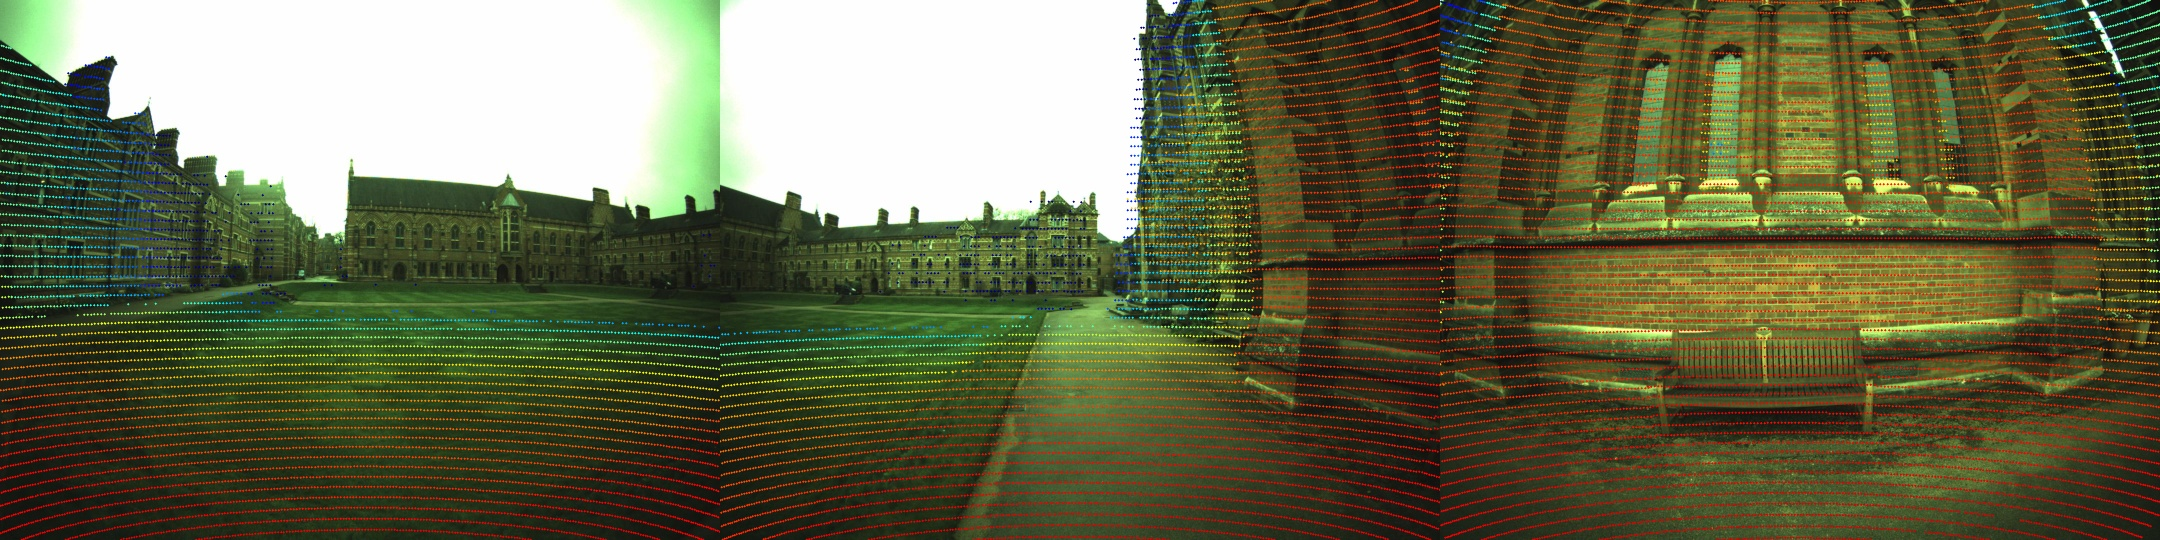
\includegraphics[width=\textwidth]{figuras/proyeccion_profundidad.jpg}\\[1mm]
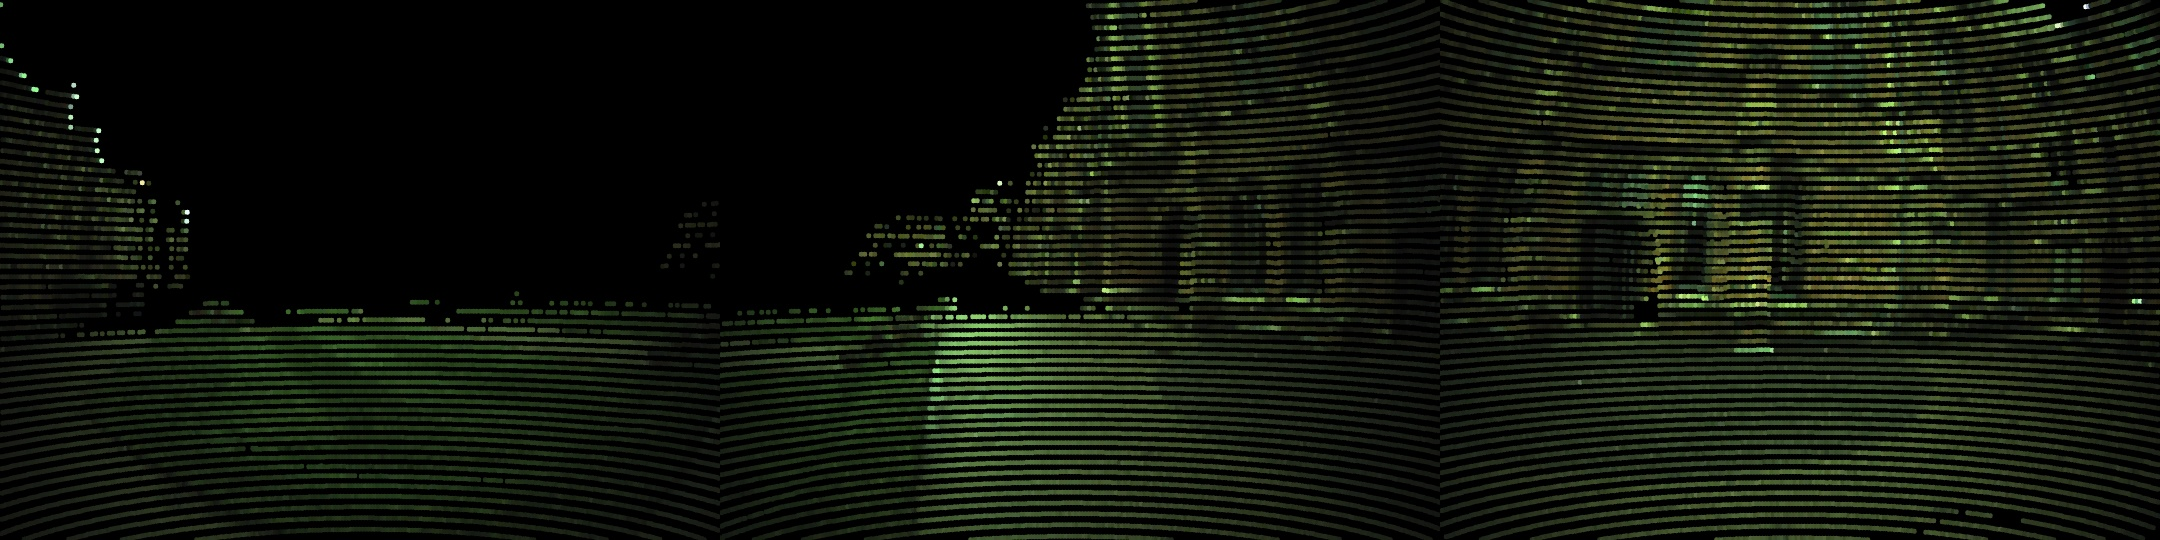
\includegraphics[width=\textwidth]{figuras/proyeccion_color.jpg}
\caption{Proyección de un barrido del LiDAR sobre las cámaras izquierda, frontal y derecha. Arriba: puntos coloreados por distancia sobre la imagen (rojo cerca, azul lejos). Abajo: los mismos puntos con el color del píxel sobre fondo negro, que corresponde al paso de coloración de la nube.}
\label{fig:proyeccion}
\end{figure*}

\subsection{Precisión de la odometría}

La trayectoria de RKO-LIO se compara con la trayectoria de referencia que proporciona el OSD para esta secuencia (\texttt{hba-tum.txt}). Las poses se asocian por \emph{timestamp} (tolerancia de 50\,ms) y se alinean en SE(3) con el método de Umeyama~\cite{umeyama1991}, sin escala, ya que el LiDAR mide en metros. Se calculan el error absoluto de trayectoria (ATE) y el error relativo de posición (RPE) sobre tramos de 10\,m~\cite{sturm2012tum}.

\begin{table}[t]
\centering
\small
\setlength{\tabcolsep}{4pt}
\begin{tabular}{@{}lcccc@{}}
\toprule
\textbf{Ejecución} & \textbf{ATE} & \textbf{ATE} & \textbf{ATE} & \textbf{RPE$_{10m}$} \\
 & \textbf{RMSE} & \textbf{máx.} & \textbf{z} & \textbf{medio} \\
\midrule
Color         & 11,5 & 36,8 & 4,0 & 9,7 \\
SegFormer v1  & 11,5 & 36,7 & 4,1 & 9,8 \\
SegFormer v2  & 11,5 & 36,7 & 4,0 & 9,8 \\
SegFormer v3  & \textbf{11,2} & \textbf{32,0} & 4,1 & \textbf{9,7} \\
YOLO11-seg    & 11,9 & 36,3 & 3,9 & 9,8 \\
\bottomrule
\end{tabular}
\caption{Error de la odometría frente a la referencia del OSD, en centímetros, sobre un recorrido de 289\,m.}
\label{tab:ate}
\end{table}

La Tabla~\ref{tab:ate} y la Figura~\ref{fig:ate} muestran los resultados. El ATE es de 11,2\,cm en un recorrido de 289\,m, con un error vertical de solo 4\,cm y un error al final del recorrido de 8\,cm; el RPE medio sobre tramos de 10\,m es de 9,7\,cm (0,97\,\%). El error es muy estable entre ejecuciones (11,2--11,9\,cm), lo que indica que la carga computacional de la segmentación no degrada la odometría. El error se mantiene acotado a lo largo de todo el recorrido, sin la deriva creciente típica de la odometría: el máximo (32\,cm) es puntual, en torno a los 190\,m. La alineación revela además que el sistema \texttt{odom} de RKO-LIO está girado unos 8$^\circ$ respecto a la vertical, porque la configuración usada no incluye fase de inicialización con la gravedad. Esto no afecta a la consistencia del mapa, solo a su orientación, y se corrige al expresarlo en el sistema de la referencia (Figura~\ref{fig:mapas}).

\begin{figure*}[t]
\centering
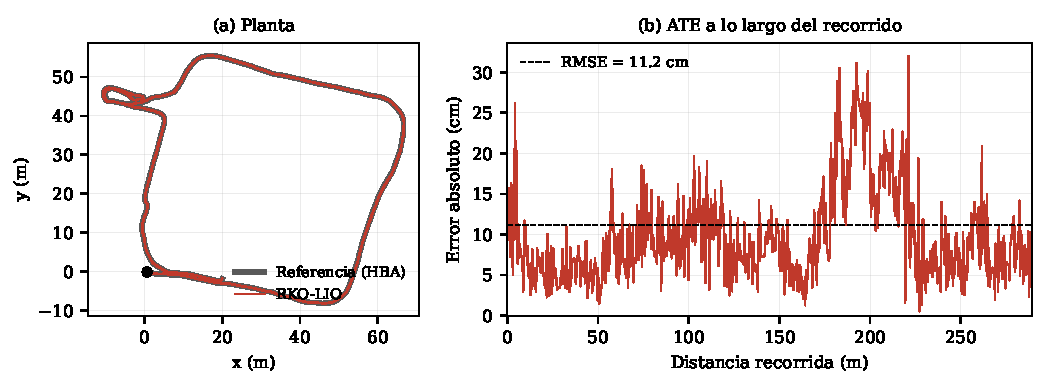
\includegraphics[width=0.92\textwidth]{figuras/ate.pdf}
\caption{(a) Trayectoria de RKO-LIO alineada con la de referencia del OSD; el punto negro marca el inicio. (b) Error absoluto a lo largo del recorrido.}
\label{fig:ate}
\end{figure*}

\subsection{Mapa geométrico y semántico}

La Figura~\ref{fig:mapas} muestra los dos mapas obtenidos, expresados en el sistema de la referencia (nivelados con la gravedad). En modo color, la nube acumulada reproduce el patio con sus caminos, el césped y las fachadas. En modo semántico, el mapa de 2,77\,M voxels queda etiquetado en su totalidad, con una confianza media del 95,5\,\%, y su estructura es coherente con la escena: edificios en todo el perímetro, calzada en los caminos que rodean el césped, terreno en los parterres, vegetación junto a las fachadas y dos vehículos aparcados.

\begin{figure*}[t]
\centering
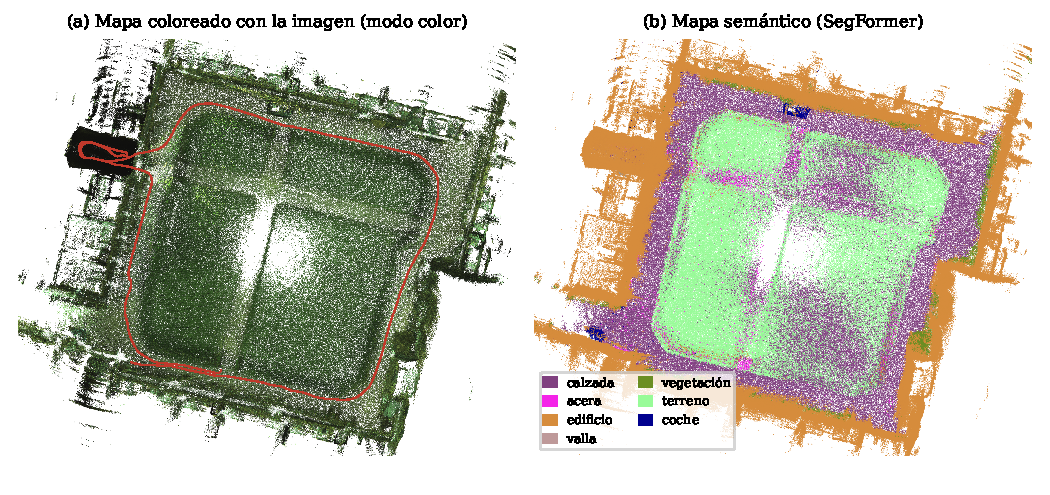
\includegraphics[width=\textwidth]{figuras/mapas_planta.pdf}
\caption{Vista en planta del patio de Keble College. (a) Mapa coloreado con las imágenes, con la trayectoria en rojo. (b) Mapa semántico obtenido con SegFormer.}
\label{fig:mapas}
\end{figure*}

El corte vertical de la Figura~\ref{fig:corte} confirma la calidad geométrica: el suelo aparece como una única capa fina, sin duplicados por deriva, y las fachadas son verticales y nítidas. El escalón entre la calzada y el césped es real, porque los parterres están por debajo de los caminos. Además, la trayectoria de referencia también presenta unos 4\,m de desnivel a lo largo del recorrido.

\begin{figure*}[t]
\centering
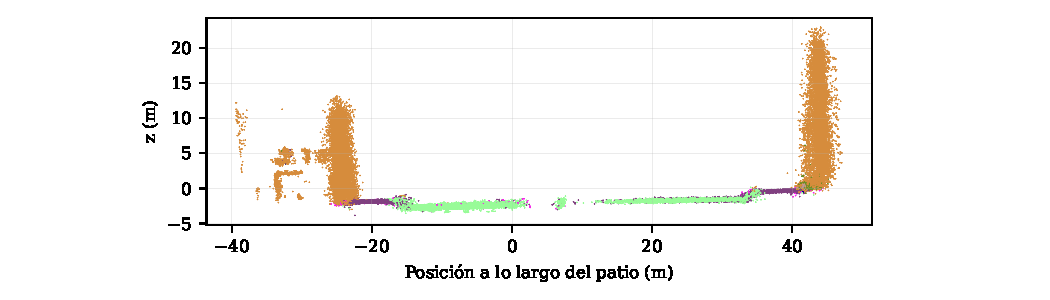
\includegraphics[width=0.92\textwidth]{figuras/corte.pdf}
\caption{Corte vertical del mapa semántico (franja de 3\,m por el centro del patio): fachadas (edificio), caminos (calzada) y césped (terreno).}
\label{fig:corte}
\end{figure*}

La Tabla~\ref{tab:clases} recoge la composición del mapa. Las clases estructurales (edificio, terreno y calzada) concentran el 95\,\% de los voxels con confianzas del 87--99\,\%. Las clases con menos confianza son las de frontera, como acera (78\,\%) y valla (75\,\%), cuya etiqueta cambia según el punto de vista. Aparecen también clases espurias con muy pocos voxels (\emph{train}, \emph{truck}, \emph{motorcycle}), que suman menos del 0,03\,\% del mapa. Las señales de tráfico son prácticamente inexistentes (4 voxels) porque la escena, un patio peatonal, apenas las contiene: es una limitación del entorno, no del sistema.

\begin{table}[t]
\centering
\small
\begin{tabular}{@{}lrrr@{}}
\toprule
\textbf{Clase} & \textbf{Voxels} & \textbf{\%} & \textbf{Confianza} \\
\midrule
Edificio   & 1\,928\,639 & 69,65 & 0,99 \\
Terreno    &   375\,875 & 13,57 & 0,91 \\
Calzada    &   336\,144 & 12,14 & 0,87 \\
Vegetación &    90\,625 &  3,27 & 0,87 \\
Acera      &    25\,662 &  0,93 & 0,78 \\
Coche      &     7\,957 &  0,29 & 0,94 \\
Valla      &     2\,848 &  0,10 & 0,75 \\
Otras (8 clases) &   1\,245 &  0,04 & -- \\
\midrule
Total      & 2\,768\,995 & 100 & 0,955 \\
\bottomrule
\end{tabular}
\caption{Composición del mapa semántico con SegFormer. La confianza es la fracción media de votos de la clase ganadora en sus voxels.}
\label{tab:clases}
\end{table}

\subsection{Segmentación densa frente a detección de objetos}

La Tabla~\ref{tab:backends} y la Figura~\ref{fig:yolo} comparan SegFormer con YOLO11-seg. YOLO solo etiqueta el 0,6\,\% del mapa, porque las clases de escena (edificio, vegetación, calzada) no existen en COCO. Detecta los mismos dos coches que SegFormer, con incluso más voxels por sus máscaras de instancia, pero también produce un falso positivo de clase \emph{train} de unos 2\,600 voxels a lo largo de una fachada. Además es más lento en este sistema, porque las máscaras se calculan a alta resolución y las imágenes se procesan de una en una, y por ello solo se integra la mitad de los barridos. La Figura~\ref{fig:clases} muestra la distribución completa de clases de ambos modelos.

\begin{table}[t]
\centering
\small
\setlength{\tabcolsep}{4pt}
\begin{tabular}{@{}lrr@{}}
\toprule
 & \textbf{SegFormer} & \textbf{YOLO11-seg} \\
\midrule
Voxels etiquetados    & 100\,\% & 0,6\,\% \\
Clases presentes      & 15 & 5 \\
Voxels de coche       & 7\,957 & 10\,229 \\
Falsos \emph{train}   & 524 & 2\,598 \\
Velocidad de segmentación   & 19,5\,img/s & 8,0\,img/s \\
Barridos integrados   & 2\,535 & 1\,493 \\
\bottomrule
\end{tabular}
\caption{Comparación de los dos backends de segmentación sobre la misma secuencia.}
\label{tab:backends}
\end{table}

\begin{figure*}[t]
\centering
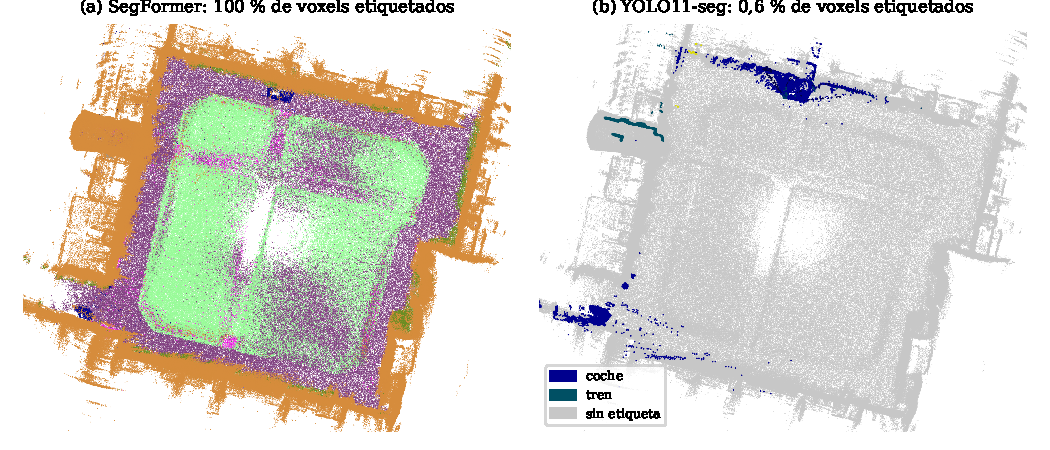
\includegraphics[width=\textwidth]{figuras/segformer_vs_yolo.pdf}
\caption{Mapa semántico obtenido con (a) SegFormer y (b) YOLO11-seg. YOLO solo etiqueta objetos discretos de COCO (vehículos), y deja sin etiqueta la estructura de la escena.}
\label{fig:yolo}
\end{figure*}

\begin{figure}[t]
\centering
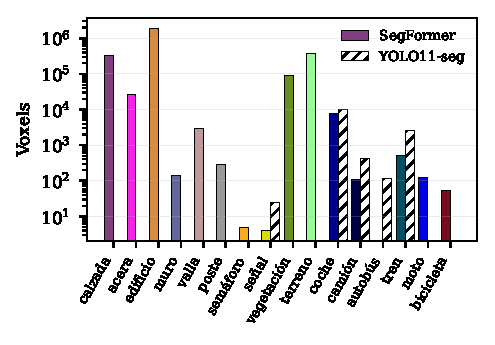
\includegraphics[width=\columnwidth]{figuras/clases.pdf}
\caption{Voxels por clase (escala logarítmica) con cada modelo.}
\label{fig:clases}
\end{figure}

La conclusión es que, para un mapa semántico de la escena completa como el que pide este proyecto, es imprescindible la segmentación semántica densa. La detección de objetos resulta útil como complemento para refinar instancias concretas.

\subsection{Rendimiento computacional}

La Tabla~\ref{tab:tiempos} recoge los tiempos medios por nodo. Todos los componentes trabajan por debajo del periodo del LiDAR (100\,ms), y el sistema integra el 84\,\% de los barridos de la secuencia reproducida en tiempo real. El resto se descarta cuando el proyector se retrasa respecto a la segmentación, lo que no afecta a la calidad del mapa debido al gran solapamiento entre barridos consecutivos.

\begin{table}[t]
\centering
\small
\begin{tabular}{@{}lr@{}}
\toprule
\textbf{Componente} & \textbf{Tiempo medio} \\
\midrule
RKO-LIO: registro ICP & 13,7\,ms \\
RKO-LIO: ciclo completo por barrido & 20,2\,ms \\
SegFormer (lote de 3 imágenes) & 153\,ms \\
Proyección y fusión de 3 cámaras & 67\,ms \\
Integración en el mapa voxelizado & 51\,ms \\
\midrule
Barridos integrados & 2\,535 / 3\,007 \\
\bottomrule
\end{tabular}
\caption{Tiempos de cómputo por componente (SegFormer v3).}
\label{tab:tiempos}
\end{table}

La Tabla~\ref{tab:optim} muestra el efecto de procesar en lotes. En la primera versión, la segmentación procesaba unas 10 imágenes por segundo, por debajo de las 30 necesarias (tres cámaras a 10\,Hz), y la mayoría de barridos se etiquetaba con una sola cámara. Con lotes multicámara y decodificación a media resolución, la segmentación sube a 19,5--23\,img/s y los puntos etiquetados por barrido pasan de unos 18\,000 a más de 40\,000, cubriendo las tres cámaras.

\begin{table}[t]
\centering
\small
\setlength{\tabcolsep}{4pt}
\begin{tabular}{@{}lrr@{}}
\toprule
 & \textbf{v1 (secuencial)} & \textbf{v2 (lotes)} \\
\midrule
Segmentación (img/s)      & $\sim$10 & 19,5--23 \\
Puntos etiquetados/barrido & $\sim$18\,000 & $\sim$43\,000 \\
Proyector (ms/barrido)    & 28 & 67--72 \\
\bottomrule
\end{tabular}
\caption{Efecto de la segmentación por lotes multicámara. El proyector tarda más en v2 porque procesa el triple de puntos.}
\label{tab:optim}
\end{table}

\subsection{Limitaciones}

\begin{itemize}[noitemsep]
  \item \textbf{Evaluación semántica indirecta.} El OSD no contiene anotaciones semánticas, por lo que la calidad semántica se evalúa con indicadores internos (confianza, consistencia), inspección cualitativa y comparación entre modelos, no con mIoU.
  \item \textbf{Oclusiones.} Al proyectar no se comprueba la visibilidad. Un punto ocluido para la cámara puede recibir la etiqueta del objeto que lo tapa; la separación de solo unos 10\,cm entre LiDAR y cámaras y la votación multivista limitan este efecto.
  \item \textbf{Movimiento durante el barrido.} Se proyecta la nube sin compensar el movimiento durante los 100\,ms del barrido ni el desfase de hasta 80\,ms con la imagen; a velocidad de marcha (unos 1\,m/s) esto supone un error de pocos centímetros, inferior al tamaño del voxel.
  \item \textbf{Vocabulario cerrado.} Las clases están limitadas a las 19 de Cityscapes.
\end{itemize}

%==========================================================
\section{Conclusiones y Trabajo Futuro}
%==========================================================

Se ha desarrollado un sistema completo en ROS~2 que interpreta semánticamente un entorno urbano combinando odometría LiDAR-inercial y segmentación de imagen con modelos preentrenados. El sistema proyecta las etiquetas de tres cámaras ojo de pez sobre el LiDAR con el modelo equidistante calibrado, y las fusiona en un mapa voxelizado mediante una votación con justificación bayesiana. Todo funciona en tiempo real y se reproduce con un único comando sobre el contenedor Docker de la asignatura.

Sobre la secuencia Keble College~01 del OSD, la odometría alcanza un ATE de 11,2\,cm en 289\,m, y el mapa semántico resultante queda etiquetado en su totalidad con una confianza media del 95,5\,\%. Su estructura es coherente con la escena real. La comparación con YOLO11-seg muestra que la detección de objetos no basta para un mapa semántico de la escena (0,6\,\% de cobertura) y justifica la segmentación densa.

Como trabajo futuro se proponen las siguientes líneas:
\begin{itemize}[noitemsep]
  \item \textbf{Modelos de vocabulario abierto.} Integrar SAM~3~\cite{carion2025sam3} como backend, para segmentar a partir de texto (<<ventana>>, <<puerta>>, <<banco>>) sin limitarse a Cityscapes.
  \item \textbf{Fusión de backends.} Usar SegFormer para la escena y YOLO o SAM para refinar instancias de objetos.
  \item \textbf{Evaluación geométrica y semántica.} Medir la precisión y completitud del mapa frente al modelo del escáner láser terrestre del OSD, y anotar un subconjunto de imágenes para obtener el mIoU.
  \item \textbf{Mejoras del pipeline.} Gestionar oclusiones con un z-buffer por cámara, compensar el movimiento durante el barrido, alinear el mapa con la gravedad desde el inicio y añadir cierre de bucle para recorridos largos.
\end{itemize}

\nocite{*}
\bibliography{custom}

\end{document}
